\noindent
I denne workshop er fokus lidt ændret fra tidligere Workshop. Dette er grundet at tidligere Workshop hovedsageligt havde fokus på projektets login funktionalitet og de dertilhørende usecases. Til denne workshop har gruppen dog vedtaget at det mere oplagt at videre specificere projektets andre dele, her tale om interaktion og implementering.

\begin{figure}[H]
    \centering
    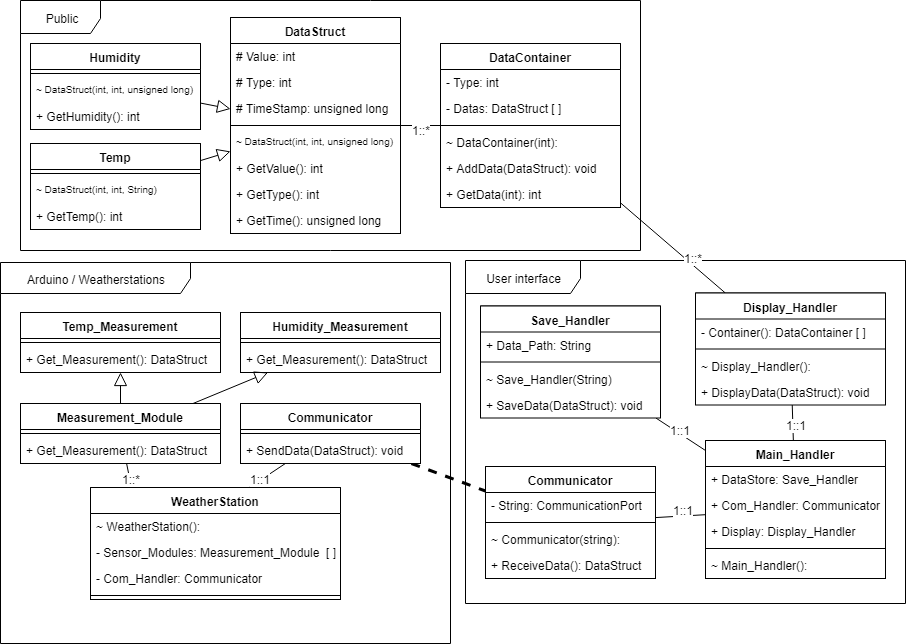
\includegraphics[width=1\textwidth, angle =0]{Struktureret_System_Udvikling/Workshop_2/Assets/Workshop2_ClassDiagram.png}
    \caption{Interaction Class Diagram}
    \label{fig:my_label}
\end{figure}

\noindent
Som ses på overstående klassediagram kan implementationen af Vejrstationen og dens kommunikation, indeles i tre generelle hovedpunkter til den videre implementation.\\
1. kaldet Public:
Der generelt beskriver funktionaliteter anvendt af både Vejrstationens egen implementation, men også af eventuelle Userinterface.
I denne kan f.eks. ses en beskrivelse af en Data Container "Data\_Struct", lavet til at kunne håndtere alle former for data sendt i en enten intern eller ekstern kommunikations forbindelse.\\
2. kaldet Arduino / Weatherstations:
Denne beskriver generelt funktionaliteten implementeret i Vejrstationen alene, dog her både til at anskaffe data, fra hvert enkelt sensor modul, men også til at håndtere, samt videresende samme data til eventuelle udestående Userinterface.\\
3. kaldet Userinterface:
Som generelt beskriver den nødvendige implementation til håndtering og visning af data'en, her modtaget fra en Vejrstation, og den videre mulige interaktion mellem platformen og brugeren.

\begin{figure}[H]
    \centering
    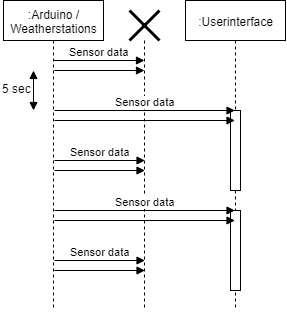
\includegraphics[width=0.4\textwidth, angle =0]{Struktureret_System_Udvikling/Workshop_2/Assets/Workshop2_SequenceDiagram.png}
    \caption{Interaction Sequence Diagram}
    \label{fig:my_label}
\end{figure}
\noindent
Vejrstationens opgave er, som vist ovenfor, at sende data hvert femte sekund, dog uden grundlag for nogen modtager. Modtageren "Userinterface" tager nemlig selv interaktiv til, efter rådighed, at modtage og bearbejde den tilgængelige data.
Dette gør at data ikke bare er tilgængelig for den enkelte modtager men mere for alle interesserede.
Til transformation af Data mellem Vejrstation og Userinterface, har gruppen valgt at opbygge følgende API:
\begin{figure}[H]
    \centering
    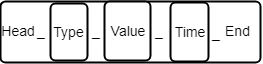
\includegraphics[width=0.3\textwidth, angle =0]{Struktureret_System_Udvikling/Workshop_2/Assets/Workshop2_DataStructure.png}
    \caption{Data Structure Blok}
    \label{fig:my_label}
\end{figure}
\noindent
Denne opbygger en struktur, der generelt kan indeholde alle typer af Vejrstationens sensor data, skelnet mellem ved datablokkens type blok.